
%% bare_jrnl.tex
%% V1.4b
%% 2015/08/26
%% by Michael Shell
%% see http://www.michaelshell.org/
%% for current contact information.
%%
%% This is a skeleton file demonstrating the use of IEEEtran.cls
%% (requires IEEEtran.cls version 1.8b or later) with an IEEE
%% journal paper.
%%
%% Support sites:
%% http://www.michaelshell.org/tex/ieeetran/
%% http://www.ctan.org/pkg/ieeetran
%% and
%% http://www.ieee.org/

%%*************************************************************************
%% Legal Notice:
%% This code is offered as-is without any warranty either expressed or
%% implied; without even the implied warranty of MERCHANTABILITY or
%% FITNESS FOR A PARTICULAR PURPOSE! 
%% User assumes all risk.
%% In no event shall the IEEE or any contributor to this code be liable for
%% any damages or losses, including, but not limited to, incidental,
%% consequential, or any other damages, resulting from the use or misuse
%% of any information contained here.
%%
%% All comments are the opinions of their respective authors and are not
%% necessarily endorsed by the IEEE.
%%
%% This work is distributed under the LaTeX Project Public License (LPPL)
%% ( http://www.latex-project.org/ ) version 1.3, and may be freely used,
%% distributed and modified. A copy of the LPPL, version 1.3, is included
%% in the base LaTeX documentation of all distributions of LaTeX released
%% 2003/12/01 or later.
%% Retain all contribution notices and credits.
%% ** Modified files should be clearly indicated as such, including  **
%% ** renaming them and changing author support contact information. **
%%*************************************************************************


% *** Authors should verify (and, if needed, correct) their LaTeX system  ***
% *** with the testflow diagnostic prior to trusting their LaTeX platform ***
% *** with production work. The IEEE's font choices and paper sizes can   ***
% *** trigger bugs that do not appear when using other class files.       ***                          ***
% The testflow support page is at:
% http://www.michaelshell.org/tex/testflow/



\documentclass[journal]{IEEEtran}
%
% If IEEEtran.cls has not been installed into the LaTeX system files,
% manually specify the path to it like:
% \documentclass[journal]{../sty/IEEEtran}





% Some very useful LaTeX packages include:
% (uncomment the ones you want to load)


% *** MISC UTILITY PACKAGES ***
%
\usepackage{ifpdf}
% Heiko Oberdiek's ifpdf.sty is very useful if you need conditional
% compilation based on whether the output is pdf or dvi.
% usage:
% \ifpdf
%   % pdf code
% \else
%   % dvi code
% \fi
% The latest version of ifpdf.sty can be obtained from:
% http://www.ctan.org/pkg/ifpdf
% Also, note that IEEEtran.cls V1.7 and later provides a builtin
% \ifCLASSINFOpdf conditional that works the same way.
% When switching from latex to pdflatex and vice-versa, the compiler may
% have to be run twice to clear warning/error messages.






% *** CITATION PACKAGES ***
%
%\usepackage{cite}
% cite.sty was written by Donald Arseneau
% V1.6 and later of IEEEtran pre-defines the format of the cite.sty package
% \cite{} output to follow that of the IEEE. Loading the cite package will
% result in citation numbers being automatically sorted and properly
% "compressed/ranged". e.g., [1], [9], [2], [7], [5], [6] without using
% cite.sty will become [1], [2], [5]--[7], [9] using cite.sty. cite.sty's
% \cite will automatically add leading space, if needed. Use cite.sty's
% noadjust option (cite.sty V3.8 and later) if you want to turn this off
% such as if a citation ever needs to be enclosed in parenthesis.
% cite.sty is already installed on most LaTeX systems. Be sure and use
% version 5.0 (2009-03-20) and later if using hyperref.sty.
% The latest version can be obtained at:
% http://www.ctan.org/pkg/cite
% The documentation is contained in the cite.sty file itself.






% *** GRAPHICS RELATED PACKAGES ***
%
\ifCLASSINFOpdf
   \usepackage[pdftex]{graphicx}
  % declare the path(s) where your graphic files are
  % \graphicspath{{../pdf/}{../jpeg/}}
  % and their extensions so you won't have to specify these with
  % every instance of \includegraphics
  % \DeclareGraphicsExtensions{.pdf,.jpeg,.png}
\else
  % or other class option (dvipsone, dvipdf, if not using dvips). graphicx
  % will default to the driver specified in the system graphics.cfg if no
  % driver is specified.
  % \usepackage[dvips]{graphicx}
  % declare the path(s) where your graphic files are
  % \graphicspath{{../eps/}}
  % and their extensions so you won't have to specify these with
  % every instance of \includegraphics
  % \DeclareGraphicsExtensions{.eps}
\fi
% graphicx was written by David Carlisle and Sebastian Rahtz. It is
% required if you want graphics, photos, etc. graphicx.sty is already
% installed on most LaTeX systems. The latest version and documentation
% can be obtained at: 
% http://www.ctan.org/pkg/graphicx
% Another good source of documentation is "Using Imported Graphics in
% LaTeX2e" by Keith Reckdahl which can be found at:
% http://www.ctan.org/pkg/epslatex
%
% latex, and pdflatex in dvi mode, support graphics in encapsulated
% postscript (.eps) format. pdflatex in pdf mode supports graphics
% in .pdf, .jpeg, .png and .mps (metapost) formats. Users should ensure
% that all non-photo figures use a vector format (.eps, .pdf, .mps) and
% not a bitmapped formats (.jpeg, .png). The IEEE frowns on bitmapped formats
% which can result in "jaggedy"/blurry rendering of lines and letters as
% well as large increases in file sizes.
%
% You can find documentation about the pdfTeX application at:
% http://www.tug.org/applications/pdftex





% *** MATH PACKAGES ***
%
\usepackage{amsmath}
% A popular package from the American Mathematical Society that provides
% many useful and powerful commands for dealing with mathematics.
%
% Note that the amsmath package sets \interdisplaylinepenalty to 10000
% thus preventing page breaks from occurring within multiline equations. Use:
%\interdisplaylinepenalty=2500
% after loading amsmath to restore such page breaks as IEEEtran.cls normally
% does. amsmath.sty is already installed on most LaTeX systems. The latest
% version and documentation can be obtained at:
% http://www.ctan.org/pkg/amsmath





% *** SPECIALIZED LIST PACKAGES ***
%
\usepackage{algorithmic}
% algorithmic.sty was written by Peter Williams and Rogerio Brito.
% This package provides an algorithmic environment fo describing algorithms.
% You can use the algorithmic environment in-text or within a figure
% environment to provide for a floating algorithm. Do NOT use the algorithm
% floating environment provided by algorithm.sty (by the same authors) or
% algorithm2e.sty (by Christophe Fiorio) as the IEEE does not use dedicated
% algorithm float types and packages that provide these will not provide
% correct IEEE style captions. The latest version and documentation of
% algorithmic.sty can be obtained at:
% http://www.ctan.org/pkg/algorithms
% Also of interest may be the (relatively newer and more customizable)
% algorithmicx.sty package by Szasz Janos:
% http://www.ctan.org/pkg/algorithmicx




% *** ALIGNMENT PACKAGES ***
%
\usepackage{array}
% Frank Mittelbach's and David Carlisle's array.sty patches and improves
% the standard LaTeX2e array and tabular environments to provide better
% appearance and additional user controls. As the default LaTeX2e table
% generation code is lacking to the point of almost being broken with
% respect to the quality of the end results, all users are strongly
% advised to use an enhanced (at the very least that provided by array.sty)
% set of table tools. array.sty is already installed on most systems. The
% latest version and documentation can be obtained at:
% http://www.ctan.org/pkg/array


% IEEEtran contains the IEEEeqnarray family of commands that can be used to
% generate multiline equations as well as matrices, tables, etc., of high
% quality.




% *** SUBFIGURE PACKAGES ***
%\ifCLASSOPTIONcompsoc
%  \usepackage[caption=false,font=normalsize,labelfont=sf,textfont=sf]{subfig}
%\else
%  \usepackage[caption=false,font=footnotesize]{subfig}
%\fi
% subfig.sty, written by Steven Douglas Cochran, is the modern replacement
% for subfigure.sty, the latter of which is no longer maintained and is
% incompatible with some LaTeX packages including fixltx2e. However,
% subfig.sty requires and automatically loads Axel Sommerfeldt's caption.sty
% which will override IEEEtran.cls' handling of captions and this will result
% in non-IEEE style figure/table captions. To prevent this problem, be sure
% and invoke subfig.sty's "caption=false" package option (available since
% subfig.sty version 1.3, 2005/06/28) as this is will preserve IEEEtran.cls
% handling of captions.
% Note that the Computer Society format requires a larger sans serif font
% than the serif footnote size font used in traditional IEEE formatting
% and thus the need to invoke different subfig.sty package options depending
% on whether compsoc mode has been enabled.
%
% The latest version and documentation of subfig.sty can be obtained at:
% http://www.ctan.org/pkg/subfig




% *** FLOAT PACKAGES ***
%
%\usepackage{fixltx2e}
% fixltx2e, the successor to the earlier fix2col.sty, was written by
% Frank Mittelbach and David Carlisle. This package corrects a few problems
% in the LaTeX2e kernel, the most notable of which is that in current
% LaTeX2e releases, the ordering of single and double column floats is not
% guaranteed to be preserved. Thus, an unpatched LaTeX2e can allow a
% single column figure to be placed prior to an earlier double column
% figure.
% Be aware that LaTeX2e kernels dated 2015 and later have fixltx2e.sty's
% corrections already built into the system in which case a warning will
% be issued if an attempt is made to load fixltx2e.sty as it is no longer
% needed.
% The latest version and documentation can be found at:
% http://www.ctan.org/pkg/fixltx2e


%\usepackage{stfloats}
% stfloats.sty was written by Sigitas Tolusis. This package gives LaTeX2e
% the ability to do double column floats at the bottom of the page as well
% as the top. (e.g., "\begin{figure*}[!b]" is not normally possible in
% LaTeX2e). It also provides a command:
%\fnbelowfloat
% to enable the placement of footnotes below bottom floats (the standard
% LaTeX2e kernel puts them above bottom floats). This is an invasive package
% which rewrites many portions of the LaTeX2e float routines. It may not work
% with other packages that modify the LaTeX2e float routines. The latest
% version and documentation can be obtained at:
% http://www.ctan.org/pkg/stfloats
% Do not use the stfloats baselinefloat ability as the IEEE does not allow
% \baselineskip to stretch. Authors submitting work to the IEEE should note
% that the IEEE rarely uses double column equations and that authors should try
% to avoid such use. Do not be tempted to use the cuted.sty or midfloat.sty
% packages (also by Sigitas Tolusis) as the IEEE does not format its papers in
% such ways.
% Do not attempt to use stfloats with fixltx2e as they are incompatible.
% Instead, use Morten Hogholm'a dblfloatfix which combines the features
% of both fixltx2e and stfloats:
%
% \usepackage{dblfloatfix}
% The latest version can be found at:
% http://www.ctan.org/pkg/dblfloatfix




%\ifCLASSOPTIONcaptionsoff
%  \usepackage[nomarkers]{endfloat}
% \let\MYoriglatexcaption\caption
% \renewcommand{\caption}[2][\relax]{\MYoriglatexcaption[#2]{#2}}
%\fi
% endfloat.sty was written by James Darrell McCauley, Jeff Goldberg and 
% Axel Sommerfeldt. This package may be useful when used in conjunction with 
% IEEEtran.cls'  captionsoff option. Some IEEE journals/societies require that
% submissions have lists of figures/tables at the end of the paper and that
% figures/tables without any captions are placed on a page by themselves at
% the end of the document. If needed, the draftcls IEEEtran class option or
% \CLASSINPUTbaselinestretch interface can be used to increase the line
% spacing as well. Be sure and use the nomarkers option of endfloat to
% prevent endfloat from "marking" where the figures would have been placed
% in the text. The two hack lines of code above are a slight modification of
% that suggested by in the endfloat docs (section 8.4.1) to ensure that
% the full captions always appear in the list of figures/tables - even if
% the user used the short optional argument of \caption[]{}.
% IEEE papers do not typically make use of \caption[]'s optional argument,
% so this should not be an issue. A similar trick can be used to disable
% captions of packages such as subfig.sty that lack options to turn off
% the subcaptions:
% For subfig.sty:
% \let\MYorigsubfloat\subfloat
% \renewcommand{\subfloat}[2][\relax]{\MYorigsubfloat[]{#2}}
% However, the above trick will not work if both optional arguments of
% the \subfloat command are used. Furthermore, there needs to be a
% description of each subfigure *somewhere* and endfloat does not add
% subfigure captions to its list of figures. Thus, the best approach is to
% avoid the use of subfigure captions (many IEEE journals avoid them anyway)
% and instead reference/explain all the subfigures within the main caption.
% The latest version of endfloat.sty and its documentation can obtained at:
% http://www.ctan.org/pkg/endfloat
%
% The IEEEtran \ifCLASSOPTIONcaptionsoff conditional can also be used
% later in the document, say, to conditionally put the References on a 
% page by themselves.




% *** PDF, URL AND HYPERLINK PACKAGES ***
%
\usepackage{url}
% url.sty was written by Donald Arseneau. It provides better support for
% handling and breaking URLs. url.sty is already installed on most LaTeX
% systems. The latest version and documentation can be obtained at:
% http://www.ctan.org/pkg/url
% Basically, \url{my_url_here}.




% *** Do not adjust lengths that control margins, column widths, etc. ***
% *** Do not use packages that alter fonts (such as pslatex).         ***
% There should be no need to do such things with IEEEtran.cls V1.6 and later.
% (Unless specifically asked to do so by the journal or conference you plan
% to submit to, of course. )


% correct bad hyphenation here
\hyphenation{op-tical net-works semi-conduc-tor}


\begin{document}
%
% paper title
% Titles are generally capitalized except for words such as a, an, and, as,
% at, but, by, for, in, nor, of, on, or, the, to and up, which are usually
% not capitalized unless they are the first or last word of the title.
% Linebreaks \\ can be used within to get better formatting as desired.
% Do not put math or special symbols in the title.
\title{A Survey of Technologies for Mobile Payment Security 
}
%
%
% author names and IEEE memberships
% note positions of commas and nonbreaking spaces ( ~ ) LaTeX will not break
% a structure at a ~ so this keeps an author's name from being broken across
% two lines.
% use \thanks{} to gain access to the first footnote area
% a separate \thanks must be used for each paragraph as LaTeX2e's \thanks
% was not built to handle multiple paragraphs
%

\author{Wenzheng Liu,~\IEEEmembership{Student,~NUDT,}
        John~Doe,~\IEEEmembership{Fellow,~OSA,}
        and~Jane~Doe,~\IEEEmembership{Life~Fellow,~IEEE}% <-this % stops a space
\thanks{M. Shell was with the Department
of Electrical and Computer Engineering, Georgia Institute of Technology, Atlanta,
GA, 30332 USA e-mail: (see http://www.michaelshell.org/contact.html).}% <-this % stops a space
\thanks{J. Doe and J. Doe are with Anonymous University.}% <-this % stops a space
\thanks{Manuscript received April 19, 2005; revised August 26, 2015.}}

% note the % following the last \IEEEmembership and also \thanks - 
% these prevent an unwanted space from occurring between the last author name
% and the end of the author line. i.e., if you had this:
% 
% \author{....lastname \thanks{...} \thanks{...} }
%                     ^------------^------------^----Do not want these spaces!
%
% a space would be appended to the last name and could cause every name on that
% line to be shifted left slightly. This is one of those "LaTeX things". For
% instance, "\textbf{A} \textbf{B}" will typeset as "A B" not "AB". To get
% "AB" then you have to do: "\textbf{A}\textbf{B}"
% \thanks is no different in this regard, so shield the last } of each \thanks
% that ends a line with a % and do not let a space in before the next \thanks.
% Spaces after \IEEEmembership other than the last one are OK (and needed) as
% you are supposed to have spaces between the names. For what it is worth,
% this is a minor point as most people would not even notice if the said evil
% space somehow managed to creep in.



% The paper headers
\markboth{Journal of \LaTeX\ Class Files,~Vol.~14, No.~8, August~2015}%
{Shell \MakeLowercase{\textit{et al.}}: Bare Demo of IEEEtran.cls for IEEE Journals}
% The only time the second header will appear is for the odd numbered pages
% after the title page when using the twoside option.
% 
% *** Note that you probably will NOT want to include the author's ***
% *** name in the headers of peer review papers.                   ***
% You can use \ifCLASSOPTIONpeerreview for conditional compilation here if
% you desire.




% If you want to put a publisher's ID mark on the page you can do it like
% this:
%\IEEEpubid{0000--0000/00\$00.00~\copyright~2015 IEEE}
% Remember, if you use this you must call \IEEEpubidadjcol in the second
% column for its text to clear the IEEEpubid mark.



% use for special paper notices
%\IEEEspecialpapernotice{(Invited Paper)}




% make the title area
\maketitle

% As a general rule, do not put math, special symbols or citations
% in the abstract or keywords.
\begin{abstract}
Nowadays, the rising penetration of smartphones and the important roles of them in people’s daily
life make the smartphones an ideal medium to conduct payment transactions. The smartphones are
capable to store everything that would normally be carried in a physical wallet and also allows the
users to make payments anytime and anywhere. The potential added-values of mobile payments,
such as generating new revenues, obtaining new users, increasing user stickiness attracted different
players to expand their businesses to the mobile payment services, including financial institutions,
mobile network operators, mobile device manufacturers, trusted third party providers. To compete
in the market, they explored different technologies and business models which resulted in the
complexity and dynamics of the mobile payment market. Consequently, mobile payments have
only become a standard practice in a few countries. In terms of proximity payments, NFC is widely
viewed as one of the most promising technologies due to its security features, compatibility with
the existing financial infrastructures, and ease of use. In the Chinese market, compared with QR
code, NFC was first introduced and supported by various players. However, the Chinese mobile
proximity payment market has become the largest and fastest-growing mobile proximity payment
market in the world in few years by utilising QR code. The market is highly concentrated with
Alipay and Tenpay which are QR code-based mobile payment platforms. In other words, QR code
overtook NFC and became the most popular mobile proximity payment technology in China.
\end{abstract}

% Note that keywords are not normally used for peerreview papers.
\begin{IEEEkeywords}
token, payment, offline, \LaTeX, online, TOTP.
\end{IEEEkeywords}






% For peer review papers, you can put extra information on the cover
% page as needed:
% \ifCLASSOPTIONpeerreview
% \begin{center} \bfseries EDICS Category: 3-BBND \end{center}
% \fi
%
% For peerreview papers, this IEEEtran command inserts a page break and
% creates the second title. It will be ignored for other modes.
\IEEEpeerreviewmaketitle



%\section{Introduction}
% The very first letter is a 2 line initial drop letter followed
% by the rest of the first word in caps.
% 
% form to use if the first word consists of a single letter:
% \IEEEPARstart{A}{demo} file is ....
% 
% form to use if you need the single drop letter followed by
% normal text (unknown if ever used by the IEEE):
% \IEEEPARstart{A}{}demo file is ....
% 
% Some journals put the first two words in caps:
% \IEEEPARstart{T}{his demo} file is ....
% 
% Here we have the typical use of a "T" for an initial drop letter
% and "HIS" in caps to complete the first word.
%\IEEEPARstart{T}{his} demo file is intended to serve as a ``starter file''
%for IEEE journal papers produced under \LaTeX\ using
%IEEEtran.cls version 1.8b and later.
% You must have at least 2 lines in the paragraph with the drop letter
% (should never be an issue)
%I wish you the best of success.

%\hfill mds
 
%\hfill August 26, 2015
\section{Introduction}
\IEEEPARstart{I}n this study, the research model is developed based on relevant business model, platform and
business ecosystem theories. The final research model consists of three connected perspectives
 Chinese mobile payment platforms, namely, He Wallet, Alipay and QuickPass which have
implemented one or several technological solutions based on NFC and QR code technologies. The
data for the case studies is collected from the semi-structured interviews and the desk research. The
results showed that although NFC technology was adopted first in the Chinese market, the enabling
devices of both consumers and merchants were not widely ready at that time for NFC technology,but good enough for QR code technology. However, the early NFC adopters (both MNOs and
financial institutions) were reluctant to make a huge investment in the enabling devices to realise
the large-scale deployment in the early stage due to the uncertainties on the technology level and
the unclear roles and benefits on the business aspect. Thereby, they missed the best time to capture
user and develop users' habit. In contrast, Alipay strategically adopted the independent service
provider mode to leverage its obtained platform resources and capabilities which significantly
contributed the mass adoption of QR code in the Chinese market. Despite QR code currently
dominated the Chinese mobile payment market, it is believed that NFC has its place in the Chinese
mobile payment market as China UnionPay adopted an open platform strategy to incorporate all
relevant players into its ecosystem to facilitate the development of NFC-based mobile payments.

\subsection{Subsection Heading Here}
Subsection text here.

% needed in second column of first page if using \IEEEpubid
%\IEEEpubidadjcol

\subsubsection{Subsubsection Heading Here}
Subsubsection text here.


% An example of a floating figure using the graphicx package.
% Note that \label must occur AFTER (or within) \caption.
% For figures, \caption should occur after the \includegraphics.
% Note that IEEEtran v1.7 and later has special internal code that
% is designed to preserve the operation of \label within \caption
% even when the captionsoff option is in effect. However, because
% of issues like this, it may be the safest practice to put all your
% \label just after \caption rather than within \caption{}.
%
% Reminder: the "draftcls" or "draftclsnofoot", not "draft", class
% option should be used if it is desired that the figures are to be
% displayed while in draft mode.
%
%\begin{figure}[!t]
%\centering
%\includegraphics[width=2.5in]{myfigure}
% where an .eps filename suffix will be assumed under latex, 
% and a .pdf suffix will be assumed for pdflatex; or what has been declared
% via \DeclareGraphicsExtensions.
%\caption{Simulation results for the network.}
%\label{fig_sim}
%\end{figure}

% Note that the IEEE typically puts floats only at the top, even when this
% results in a large percentage of a column being occupied by floats.


% An example of a double column floating figure using two subfigures.
% (The subfig.sty package must be loaded for this to work.)
% The subfigure \label commands are set within each subfloat command,
% and the \label for the overall figure must come after \caption.
% \hfil is used as a separator to get equal spacing.
% Watch out that the combined width of all the subfigures on a 
% line do not exceed the text width or a line break will occur.
%
%\begin{figure*}[!t]
%\centering
%\subfloat[Case I]{\includegraphics[width=2.5in]{box}%
%\label{fig_first_case}}
%\hfil
%\subfloat[Case II]{\includegraphics[width=2.5in]{box}%
%\label{fig_second_case}}
%\caption{Simulation results for the network.}
%\label{fig_sim}
%\end{figure*}
%
% Note that often IEEE papers with subfigures do not employ subfigure
% captions (using the optional argument to \subfloat[]), but instead will
% reference/describe all of them (a), (b), etc., within the main caption.
% Be aware that for subfig.sty to generate the (a), (b), etc., subfigure
% labels, the optional argument to \subfloat must be present. If a
% subcaption is not desired, just leave its contents blank,
% e.g., \subfloat[].


% An example of a floating table. Note that, for IEEE style tables, the
% \caption command should come BEFORE the table and, given that table
% captions serve much like titles, are usually capitalized except for words
% such as a, an, and, as, at, but, by, for, in, nor, of, on, or, the, to
% and up, which are usually not capitalized unless they are the first or
% last word of the caption. Table text will default to \footnotesize as
% the IEEE normally uses this smaller font for tables.
% The \label must come after \caption as always.
%
%\begin{table}[!t]
%% increase table row spacing, adjust to taste
%\renewcommand{\arraystretch}{1.3}
% if using array.sty, it might be a good idea to tweak the value of
% \extrarowheight as needed to properly center the text within the cells
%\caption{An Example of a Table}
%\label{table_example}
%\centering
%% Some packages, such as MDW tools, offer better commands for making tables
%% than the plain LaTeX2e tabular which is used here.
%\begin{tabular}{|c||c|}
%\hline
%One & Two\\
%\hline
%Three & Four\\
%\hline
%\end{tabular}
%\end{table}


% Note that the IEEE does not put floats in the very first column
% - or typically anywhere on the first page for that matter. Also,
% in-text middle ("here") positioning is typically not used, but it
% is allowed and encouraged for Computer Society conferences (but
% not Computer Society journals). Most IEEE journals/conferences use
% top floats exclusively. 
% Note that, LaTeX2e, unlike IEEE journals/conferences, places
% footnotes above bottom floats. This can be corrected via the
% \fnbelowfloat command of the stfloats package.
\section{Virtual Bank card binding technology}
Virtual bank card instead of the real bank card binding in the payment account or mobile terminal and transfer in the transaction.In this section,the Virtual bank card binding technology will be told. First, It is need to know why the virtual bank card need bindind in the mobile phone.Accoding to the PCI DSS and China UnionPay standard,there three main reasons need to explain.
First,If the magnetic stripe card is skipped, it can be easily copied into a fake card, which is used for fraudulent transactions and brings about capital losses to the cardholder.in addition,If the card number is expired and the validity period, it is easy to move in some e-commerce in fraudulent transactions, bringing the cardholder money losses.moreover,In the online payment and mobile payment environment,the card organization is even more hopeful that it will not change the usage habit of the cardholder completing the transaction with the card number and expiration date, and at the same time effectively improve the payment security.
\subsection{The process of binding bank card.}
The payment provider hands over the bank card account (PAN) which the user needs to bind to the corresponding bank server. If the corresponding virtual bank card for this PAN does not exist for this merchant in the public central database,a new virtual is generated and an entry is added to the public central database.At the same time return virtual bank card to the merchant. The merchant binds the token with the user's account as a virtual bank card corresponding to the PAN.

However, in order to prevent the payment provider to saving or leaking the user's real bank card information, Alipay has proposed a new virtual bank card binding scheme:

1, the merchant system pre-save the payment system server authorization certificate. And authorize the signature of the authorization certificate called its default instructions.

2. The merchant system receives a binding request sent by a terminal, where the binding request corresponds to a user account that the user logs in on the merchant system; and returns a preset instruction to the terminal;

3, the terminal to the payment system through the secure channel to send the default instructions and the real bank card number.

4, the payment system generates a virtual bank card number corresponding to the real bank card number. (For each real bank card number generated by the virtual card number is different)

5, the virtual bank card number returned to the terminal.

6, the terminal sends the virtual bank card number to the payment provider.

7, the payment provider bind the virtual bank card to the user accounts.

In this scheme, the payment provider can not get the user's real bank card account information.

\begin{figure}[htbp]
\centerline{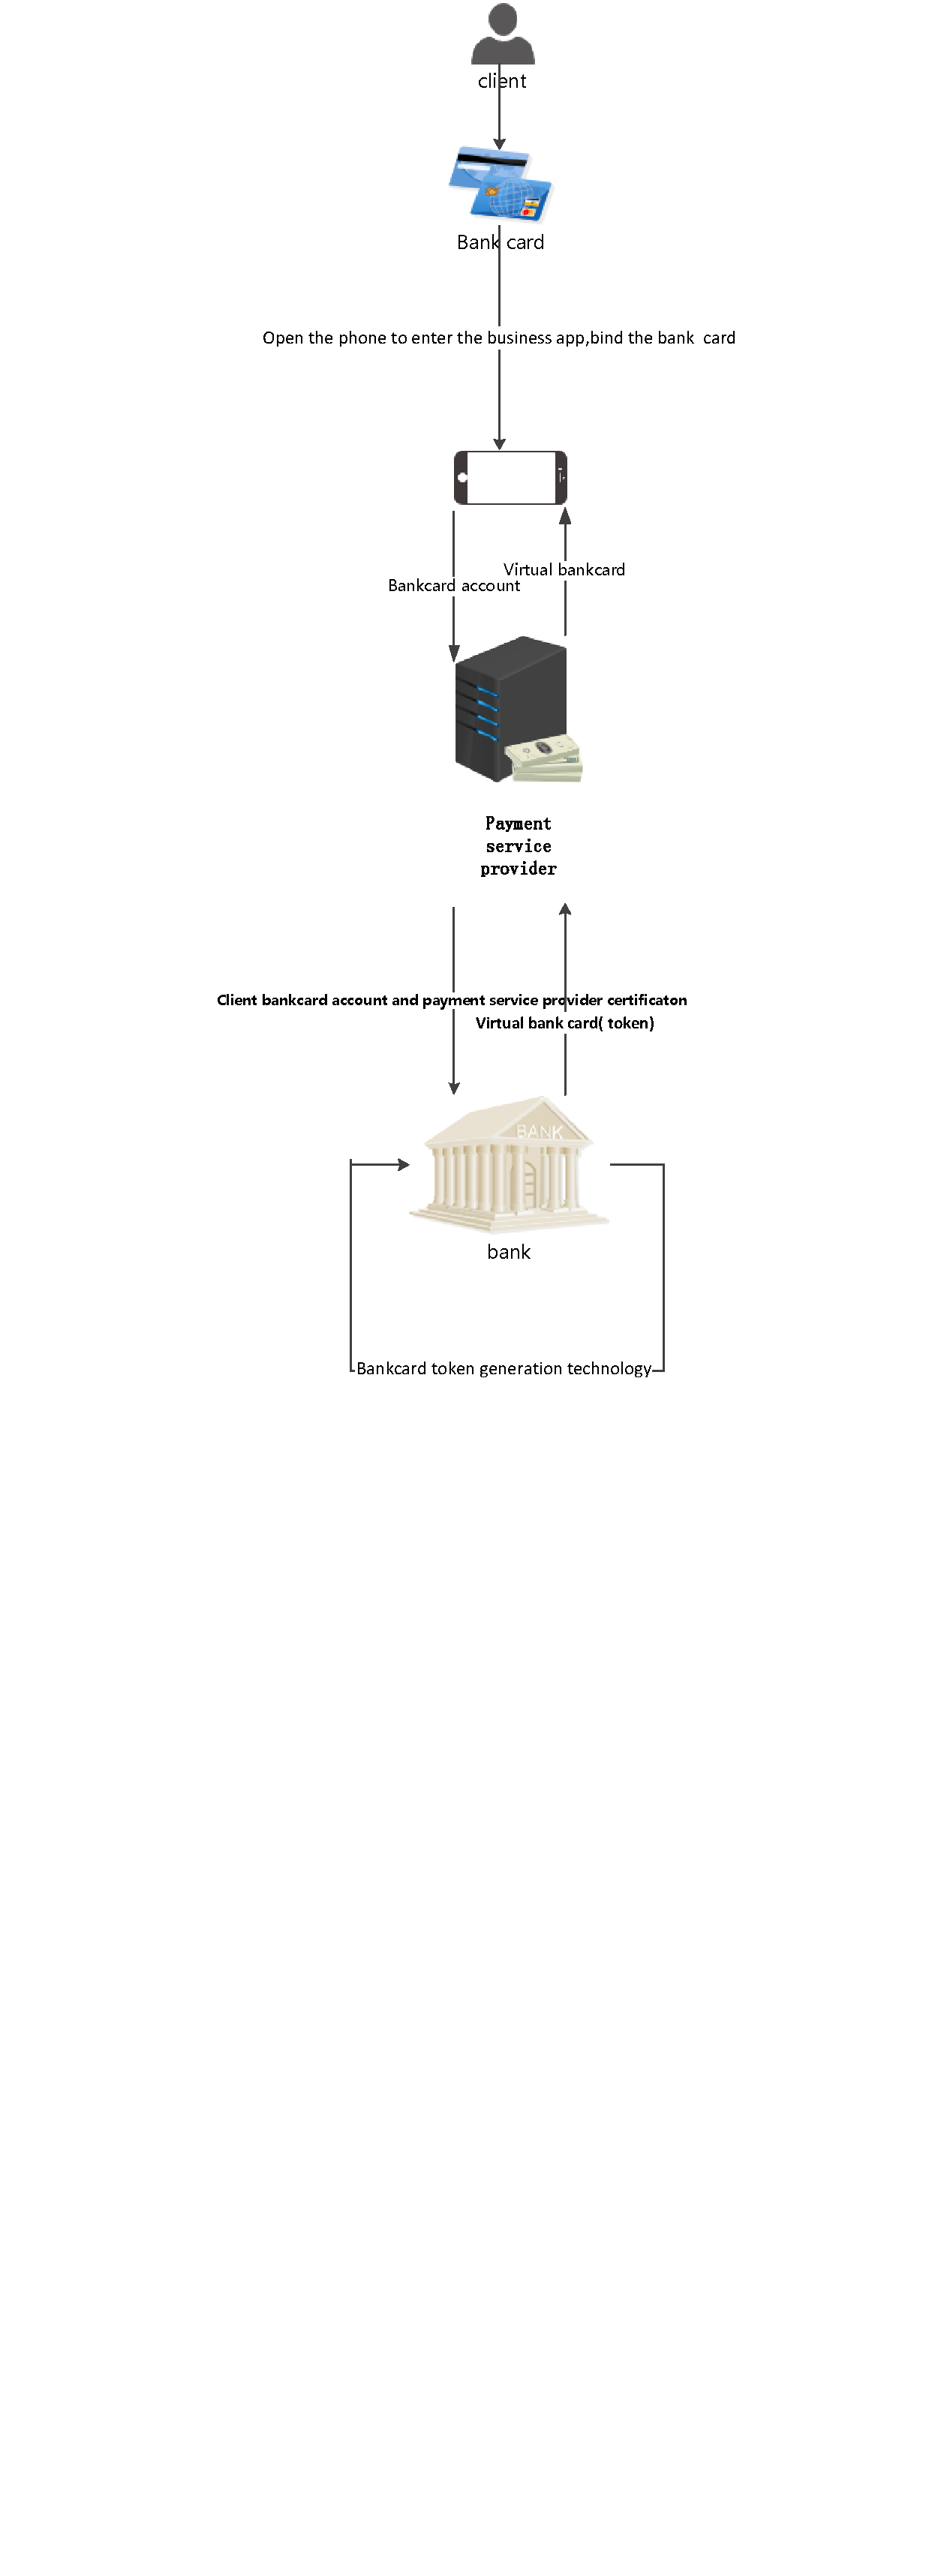
\includegraphics[scale=0.7]{token_shengcheng2.pdf}}
\caption{Token application process.}
\label{fig}
\end{figure}

\subsection{Fundamental of virtual bank card: payment tokenization }
Enterprises, merchants, and payment processors face severe, ongoing challenges securing their networks and high-value sensitive data such as payment cardholder data, to comply with the Payment Card Industry Data Security Standard (PCI DSS) and data privacy laws. Tokenization, which is used as a way of replacing sensitive data like credit card numbers with tokens, is one of the data protection and audit scope reduction methods recommended by the PCI DSS. 

The principle is to verify the transaction by using a payment token instead of a real bank card number so as to prevent card number information leakage risk. Payment tokenization is the process of replacing a traditional bank card master account with a unique numeric value, while ensuring that the value's application is limited to a specific merchant, channel, or device. Payment tags can be used in all aspects of bank card transactions, and existing bank card number based on the same transaction, can be used across industries in the industry, has versatility.
As the latest cutting-edge technology in the global payment field, payment tokenization technology has its advantages in three aspects:

First, there is no need to retain sensitive information, cardholder card number and the validity of the card does not appear in the transaction;

Second, payment tags can only be used in a limited transaction scenario, making payments more secure;

Thirdly, compared with the traditional bank card verification function, the payment tag integrates the functions of personal identification and device information verification, additional verification of payment information and risk rating to conduct transaction legitimacy identification and risk control. Therefore, the tokenization of the payment can not only prevent the leakage of sensitive information of cardholders in all aspects of transaction, but also reduce the probability of fraudulent transactions.

\begin{figure}[htbp]
\centerline{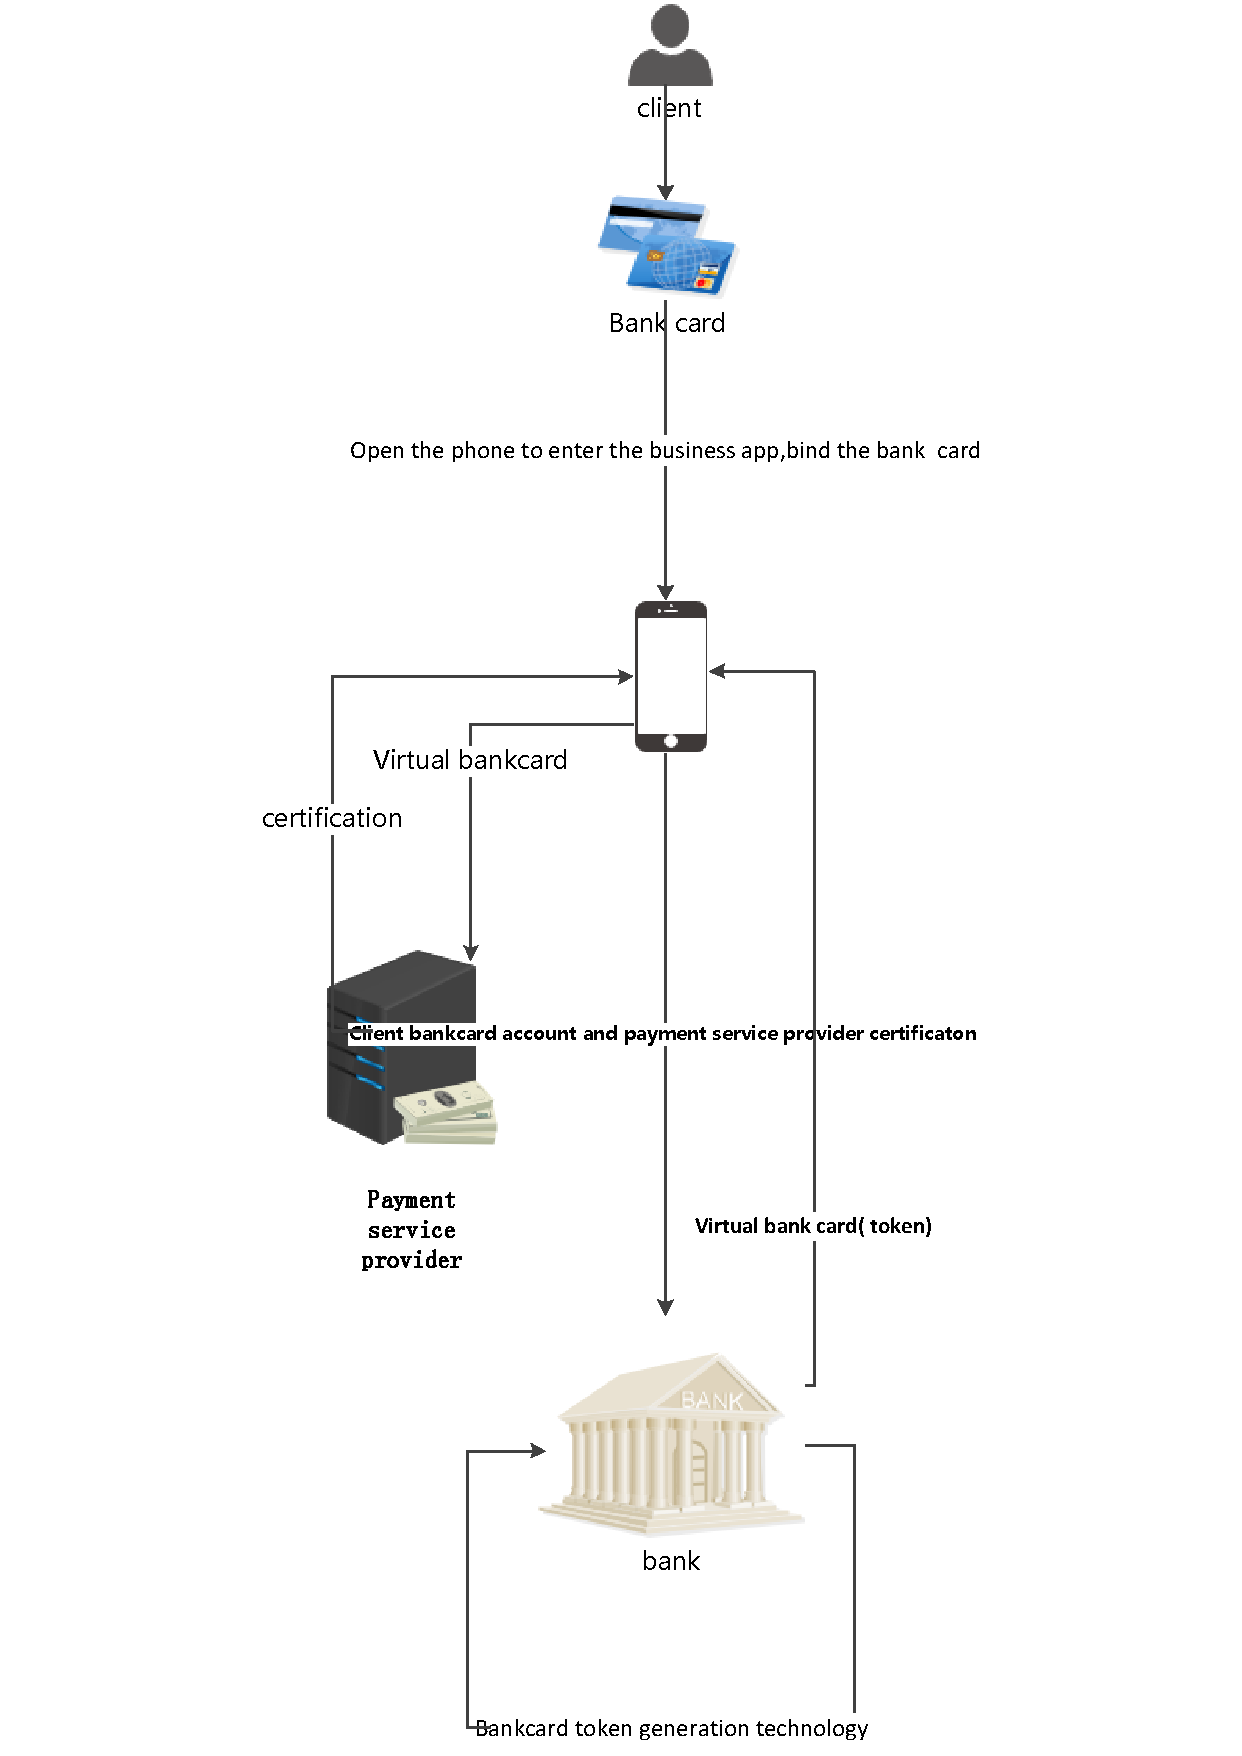
\includegraphics[scale=0.7]{token_shengcheng.pdf}}
\caption{Token application process.}
\label{fig}
\end{figure}

\subsubsection{Centralized tokenization technologies}
Centralized tokenization is conventional, database-centric solutions,which requst the token corresponding to the provided PAN from a common central database. If no token corresponding token exists in the common central database at the time of the request, a new token is generated and an entry will be added to the common central database.


\begin{figure}[htbp]
\centerline{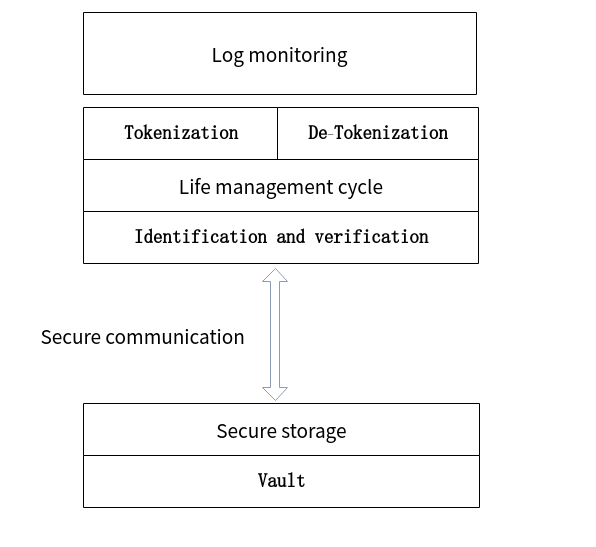
\includegraphics[scale=0.4]{tsp.png}}
\caption{token service provider}
\label{fig}
\end{figure}
 
Card organizations are highly recommended centralized tokenization technologies. 
Centralized tokenization involves building a large-scale database (“token vault”), storing each PAN together with a generated token. Figure 3 shows the China UnionPay payment tokenization system framework

\begin{figure}[htbp]
\centerline{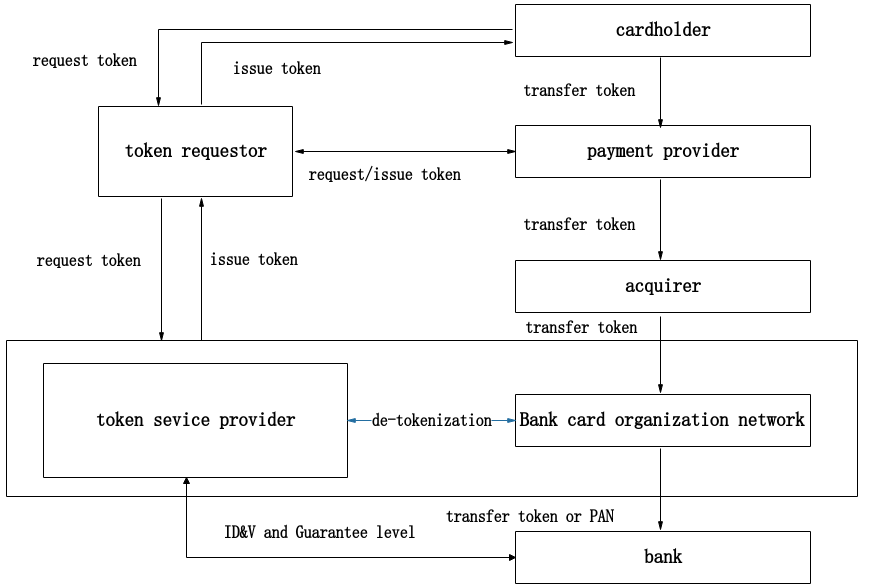
\includegraphics[width=9.5cm,height=7cm]{zhifubiaojikuangjia.png}}
\caption{China UnionPay payment tokenization system framework}
\label{fig}
\end{figure}

\subsubsection{Distributed tokenization technologies}
\section{Communication method}
Mobile payment communication is mainly used for short-distance communication, especially for poor mobile network environment offline payment. Payment information is delivered via these means of communication. Many people regard communication as a means of payment. However, they are only responsible for transmitting payment information. The real means of influencing payment are payment encryption and authentication technologies.
\subsection{QR code}
QR code is a matrix QR code symbol that was invented in 1994 by Denso Wave, a Toyota subsidiary of Japan. The QR code not only has large information capacity, high reliability, and low cost, but also can represent various character information such as Chinese characters and images, and has strong security against fraud and is very convenient to use. Therefore, it quickly became popular in Japan and South Korea. Since then, European and American countries have begun to use it in large quantities. 

QR code payment is very popular in China, people can almost go out without wallets and bank cards. You only need to show the QR code on your mobile phone to be able to pay in most places even without network. However, why is it possible to authorize payment with the QR code?

The QR code itself cannot make payment authorization, since the actual payment authorization is the payment certificate which encoded in the QR code. The payment certificate is a series of digits. You can authorize payment with this numbers. So the role of the QR code in mobile payment is to transmit this series of numbers. The specific technology of payment certificate will be told in section 4.



\subsection{NFC:MST}
Near field communication (NFC) is a wireless technology operating in the short range of four to ten centimeters for communication. It is based on radio frequency identification (RFID) technology. For a communication, an NFC device generates a radio frequency in 13.56 MHz spectrum. A receiver could receive the data through the principle of magnetic inductive coupling if it lies in a close proximity. Transmitter and receiver are small chipsets which are able to be embedded in devices such as mobile phones, POS (Point Of Sale) terminals, cards posters and many other items. 

The NFC forum (www.nfcforum.org) was formed in 2004 aimed at standardizing NFC technology. It defines NFC as: NFC is a short-range wireless connectivity technology (also known as ISO 18092) that provides intuitive, simple, and safe communication between electronic devices. Operating at the frequency of 13.56 MHz and limited short range communicating distance, NFC supports data rate of 106 Kbps, 212 Kbps and 424 Kbps. Therefore, NFC is suitable for transmission of short information or messages within small time interval. 

In recent days, NFC technology is being widely popular among mobile phone vendors and related fields. This is because NFC is compatible with already existing popular technologies such as RFID, smartcards and contactless cards. It means that stores and systems equipped with the existing technologies should not replace their infrastructure in order to support NFC. 

The incorporation of NFC into mobile devices has augmented capability of mobile phones and it is predicted to have potential to do more. This phenomenon has brought forward various works in terms of NFC transactions. At the same time, however, there are serious concerns in different terms such as privacy, user satisfaction, speed, usability, etc. Moreover, it is replacing various popular devices such as RFID tags. Hence, it is important to evaluate the performance of NFC technology and where it stands. In this paper, we have presented the brief insight to NFC technology and analyzed its performance as a mobile payment solution in terms of various factors. The mobile payment means passing of funds to vendor/merchant by customer to confirm the payment. The term “mobile” is used to represent the means to be able to move freely and easily.

\begin{figure}[htbp]
\centerline{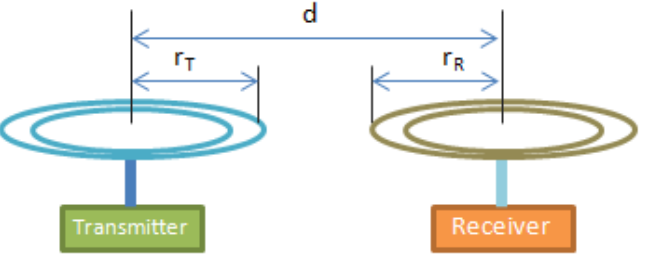
\includegraphics[scale=0.35]{InductivelycoupledNFCantennas.png}}
\caption{A complete sound packet.}
\label{fig}
\end{figure}

NFC devices communicate through the magnetically induced signals. Therefore, duringtransmission, energy is coupled between transceivers instead of electromagnetic radiation as in traditional wireless communication. The magnetic induction is discussed in detail in []. The magnetic induction theory and its application to NFC are also discussed. Figure 4 shows inductively coupled NFC antennas separated by short distance usually in the units of centimeters. Within close proximity, information can be exchanged between these transceivers by magnetic induction. Equivalent circuit diagram of these antennas is shown in Figure 5.Mathematical derivation of power at the receiver for given circuit is derived in [2], where power at the receiver can be expressed as

\begin{figure}[htbp]
\centerline{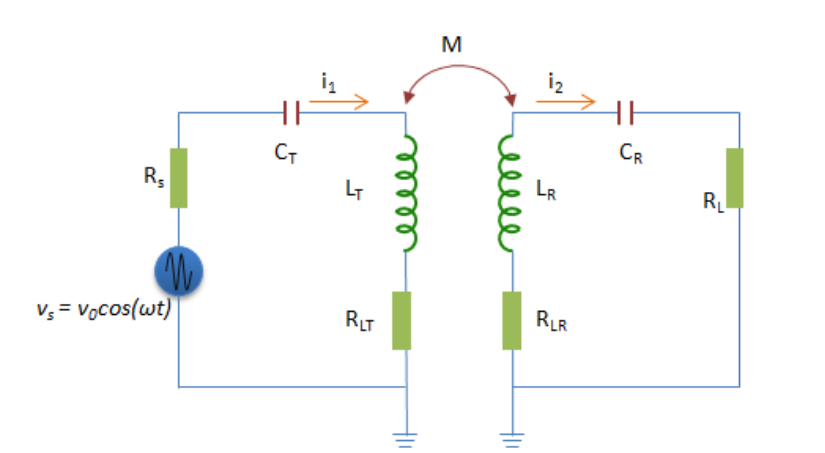
\includegraphics[scale=0.3]{EquivalentcircuitofinFigur1.png}}
\caption{A complete sound packet.}
\label{fig}
\end{figure}

$$ P_{R}(\omega)=P_{T}Q_{T}Q_{R}\eta_{T}\eta_{T}(r_{T}^{3}\mu_{0}\mu_{R}r_{R}^{3}\mu_{0}\mu_{R}\pi^{2})/(r_{T}^{3}+d^{2})^{3}.$$

where 

$P_{T}$    :Transmission power,
           
$Q_{T},Q_{R}$           : Q-factors of transmitter and receiver antenna,
          
$\eta_{T},\eta_{R}$    : Efficiency of transmitter and receiver antenna,              
                      
$r_{T},r_{R}$            : Efficiency of transmitter and receiver antenna,
           
$\mu_{0}$                          : Radii of transmitter and receiver antenna coil,
           
$\mu_{r},\mu_{R}$                        : Permeability of air (=1),
           
$D$           : Relative permeability of transmitter and receiver antenna coil core, and Distance between transmitter and receiver antenna.

An NFC system basically consists of three components as shown in Figure 5. This is the typical casewhen an NFC phone reads an NFC tag and communicates with the backend server [3-5]. In some cases, NFC tag can be another NFC phone or also there would be no need to contact backend server [6-7]. In essence, an NFC mobile system consists of an NFC tag, an NFC chip embedded mobile phone
and a backend server.

MST is "Magnetic Secure Transmissions". The technology was developed and patented by LoopPay. Samsung previously acquired the company to deploy its Samsung Pay service.The biggest highlight of Samsung Pay and Apple Pay is support for magnetic stripe card payments.

Figure 3 shows the components of the payment accessory that LoopPay made for Samsung. By using AC current, the coil will generate a magnetic field.If the correct magnetic field is generated, the coil can communicate with a credit card reader.In fact, the principle of MST is to emit a magnetic field.

\begin{figure}[htbp]
\centerline{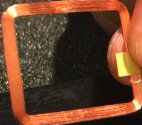
\includegraphics[scale=1]{MSTyuanjian2.png}}
\caption{token service provider}
\label{fig}
\end{figure}

However, payment security is not solved by a copper coil.The MST application has three protection mechanisms: Payment Tokenization, eSE (hardware security module) bank card information protection, KNOX, and fingerprint/password authentication.

For Token, the user needs to enter the card information and send it to the card organization for verification. After the card organization passes the verification, a token will be generated for this card and the token will be sent to the device. The credit card information is not directly stored on the device. Token is stored in an independent security chip (SE chip) and used to replace the bank card number. It can be understood that the Token and the bank card number are equivalent, but even if the Token leaks, the bank card information cannot be reversed. Only when fingerprint or password authentication passes can the token be read out through the MST. Token's storage and management is governed by Samsung's own KNOX security platform.High-risk behaviors such as equipment modification occur, and KNOX can invalidate sensitive data on the device.

In other words, when using Samsung Pay's magnetic card payment mode, the key technical step is how this Token is sent. The MST generates a dynamic magnetic field through an induction coil and can be changed according to the user-defined time limit. If your mobile device is within 3 inches of the reader, you will be able to identify the magnetic field.

Like a traditional credit or debit card, magnetic fields include your payment information. The magnetic field only exists when the user chooses to send the payment information, and the magnetic field will automatically disappear once the distance between the mobile device and the reader exceeds 3 inches. This means that the attacker must be very close to the payment process to steal the payment data.


\begin{figure}[htbp]
\centerline{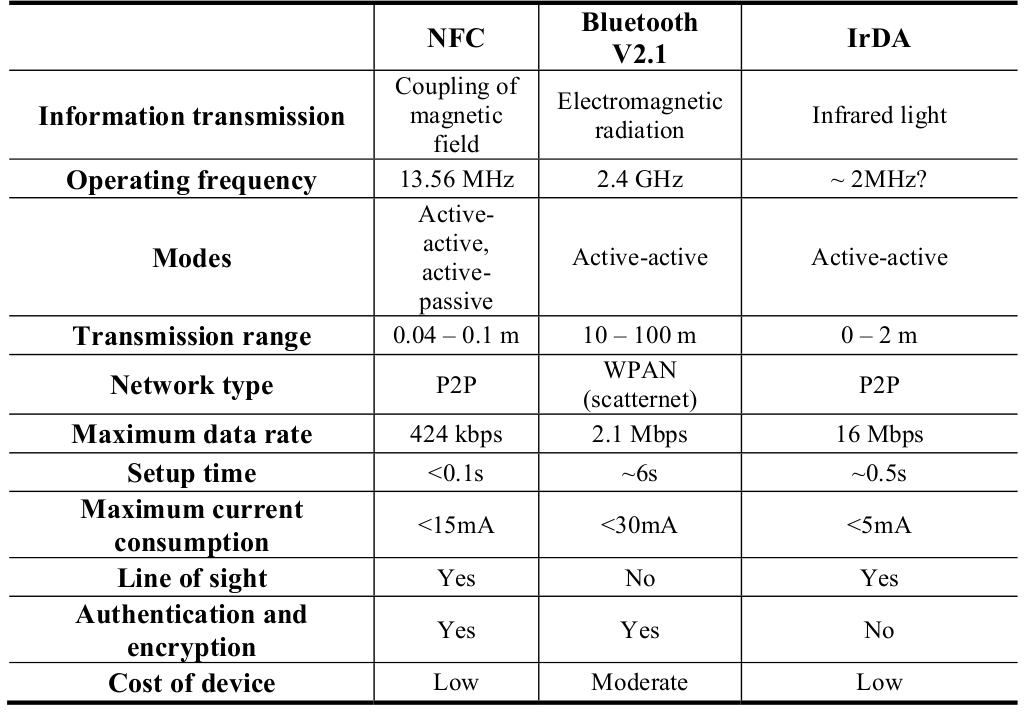
\includegraphics[scale=0.25]{ComparisonoNFCandotherPANtechnologies.png}}
\caption{Comparison of NFC and other PAN technologies}
\label{fig}
\end{figure}

An NFC system basically consists of three components as shown in Figure 5. This is the typical case when an NFC phone reads an NFC tag and communicates with the backend server [4-6]. In some cases, however, NFC tag can be another NFC phone or also there would be no need to contact backend server [7-8]. In essence, an NFC mobile system consists of an NFC tag, an NFC chip embedded mobile phone and a backend server.

An NFC tag is generally embedded in items (from which it can be read) such as smart posters [4],POS, electronic devices, etc. It is a small chip usually hidden behind a sticker with NFC logo on it in order to make users aware of its existence. These tags usually contain small data based on their applications such as uniform resource identifiers (URIs), contact information, authentication credentials, valuable information, etc.

NFC chips are embedded within mobile hand-sets enabling them to read NFC tags. Mobile phone industry has shown several NFC mobile phones manufactured in last few years. It is also possible to include NFC chip within Subscriber Identity Module (SIM) card or even in micro SD cards. Therefore, hand-sets manufactured without NFC chips from industry can also be made ‘NFC-equipped’ by inserting NFC-SIM or NFC-micro SD cards.

The NFC phones have several applications installed to utilize NFC capabilities based on the implementation of the system. It can also emulate existing cards such as credit cards, point cards, identity cards etc to give experience of these traditional schemes within a single mobile phone. Hence, a user is give experience of having 'everything' within their mobile device.

NFC phone could communicate to the backend server through different mobile communication technology. Service provided by the backend server might vary according to applications. For an instance, it could be a simple web page for reserving movie ticket, issuing receipts, or highly secure financial transaction service. Therefore, communication between handsets and backend server needs to implement secure connection.

Similar to RFID, NFC can also communicate on active/passive mode [9]. This means that an active NFC device is the one with power supply and generates radio field. The NFC device working on passive mode gets power supply through the active devices radiation. On the other hand, both the NFC devices can also work in active/active mode where both the devices are active devices with their own power supply. Generally, NFC can operate on three modes [4].

An NFC enabled phone acts as a tag or a kind of contactless card in card emulation mode. These tags can be read by existing traditional card readers. For an instance, it can be used as an identity card at school or office to unlock door, activate personal devices such as PC, printers, etc. Also, most
common usage would be to emulate credit cards or points cards which can be used at POS terminals for
payments.

An NFC has a predefined data format called NDEF data format. When an NFC phone is in read/write mode, it can read from or write data to supported tag types. Particular example usage of read/write mode is to access URI from smart posters, download short manuals of electronic devices, check out bus - arrival information at bus stops, etc.

The peer to peer mode adds quality functionality to NFC phones. In this mode, two NFC phones can exchange data with each other when brought to close proximity. For an example, two business partners can transfer their virtual business cards with each other by bringing their NFC-enabled phones close to
each other. Another popular usage is for connection handoff to other standard technology; NFC connection can be used to set-up Bluetooth pairing or Wi-Fi setup. After successful setup, the handset can use the Bluetooth or Wi-Fi connections.
\begin{figure}[htbp]
\centerline{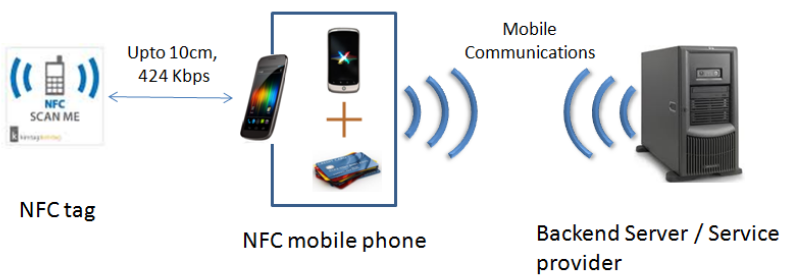
\includegraphics[scale=0.3]{NFCinactive.png}}
\caption{NFC in active/passive mode}
\label{fig}
\end{figure}


\subsection{Audio}

The audio protocol we are talking about today for sonic communication is generally from the technical documentation of chirp which is a novel application for "transmitting" files via voice issued by the American startup Animal Systems.

Acoustic wave transmission is a set of technical solutions that use sound to achieve fast transmission of files: Cross-platform technology is used to implement data transmission between any device that can send sound waves and receive sound waves.There are also a large number of applications in mobile payments.

\subsubsection{coding}
The principle of the audio protocol is simple and easy to implement. Create a table with 32 characters and map each character to a frequency table. The frequency table is generated based on the music theory through the calculation of sound.Each character is represented by the pitch of one frequency, so there are 32 frequencies, 0 corresponds to 1760 Hz, 1 corresponds to 1864 Hz,..., v corresponds to 10.5 kHz, and the adjacent frequency differs by a half interval.

The audio produced by Chirp contains 20 characters. Each character is generated with a sine wave of the corresponding frequency. Each sine wave lasts 87.2 ms. If the sampling rate is 44.1 kHz, then each character is about 3846 samples. The whole audio is about 20*87.2ms=1.744s, because each character is represented by a different frequency, it sounds like music.

A complete sound packet contains 20 tones (ie 20 characters), one tone every 87.2 milliseconds. The first two bits are headers and use “hj” to notify the receiver to start receiving. The middle 10 bits are valid information bits, which are effective transmission information, that is, Key values are mapped after the frequency information. The last 8 bits are the RS check digits. The RS parity check algorithm calculates the middle 10 bits and generates 8-bit parity information.

\begin{figure}[htbp]
\centerline{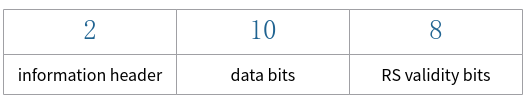
\includegraphics[scale=0.4]{yinpinwei.png}}
\caption{A complete sound packet.}
\label{fig}
\end{figure}

\subsubsection{decoding}

Chirp describes the technical details of relying on sound for data communication between a smart device, but in fact, the audio protocol of the sound wave communication can be arbitrarily designed by itself, for example, changing the sound in the chirp audio protocol to double-frequency sound, even multi-tone sound. In order to increase the information capacity per unit time, thereby increasing the transmission speed, this is all possible, as long as there is a demand for this application.

The receiver needs to record the sound and perform it and fault-tolerant processing. Its relatively high requirements on the algorithm, noise reduction and fault-tolerant processing are critical to the correct information

\section{Internet transfer payment technologies}

\begin{figure}[htbp]
\centerline{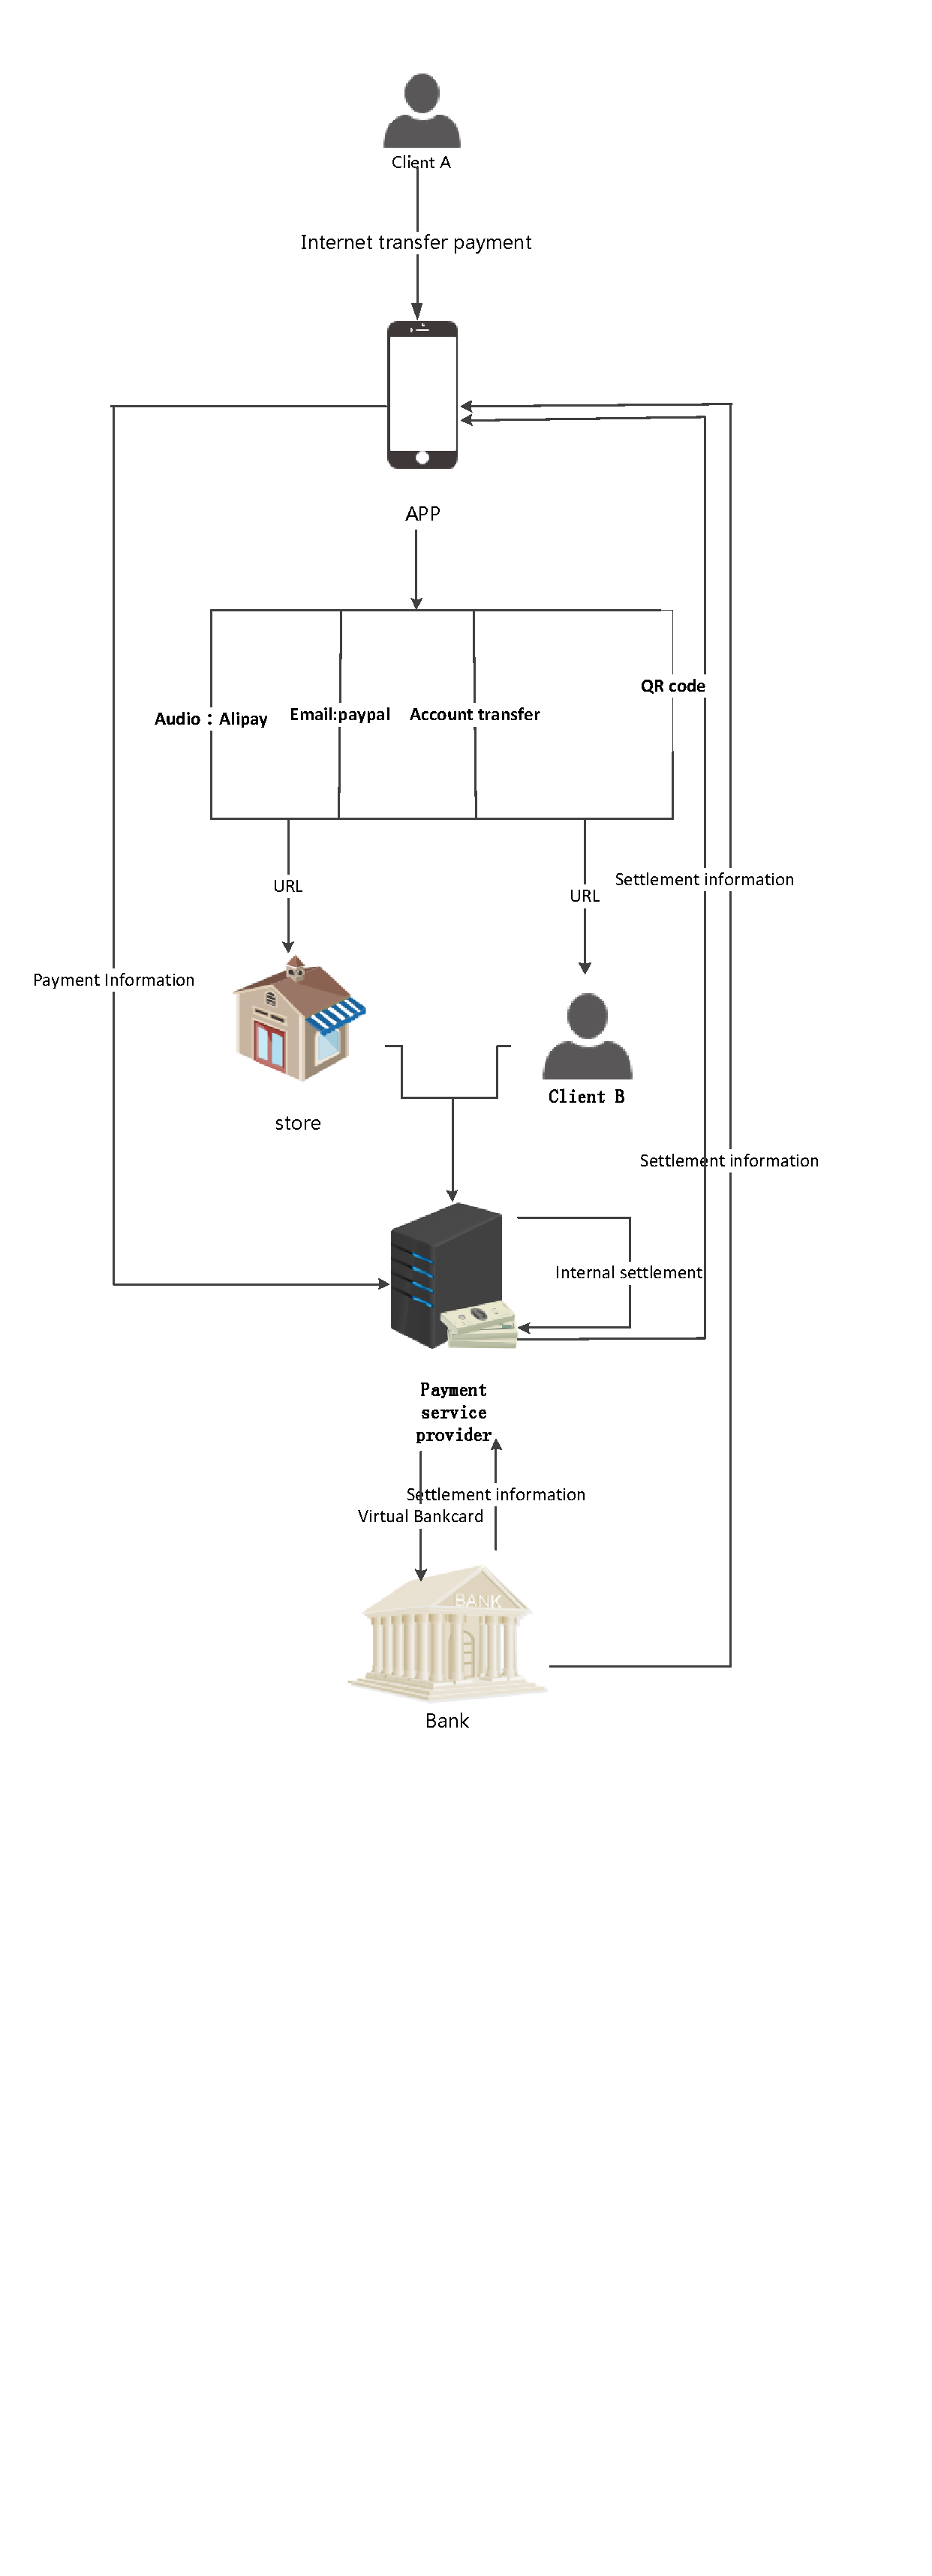
\includegraphics[scale=0.6]{zhuanzhangshifu.pdf}}
\caption{Token application process.}
\label{fig}
\end{figure}


Internet transfer payment technology, as the name suggests, is a transfer payment via the Internet.Different from the PC terminal, the network transfer payment at the mobile terminal needs to pay for the support of the client's app.

Network transfer payment technology is mainly based on the security of tokenization technology.



\subsection{scan the QR code}
In the scan code payment scenario, the QR code is actually a url with some parameters. The scan code will initiate the transfer. The two-dimensional code is actually only an account medium, a data storage body, which itself is not the result of the payment innovation. The existing various QR code payment only replaces the data carrier of the original payment means with a two-dimensional code. Similar chip content with bank cards. Is an account of the embodiment. 
\begin{figure}[htbp]
\centerline{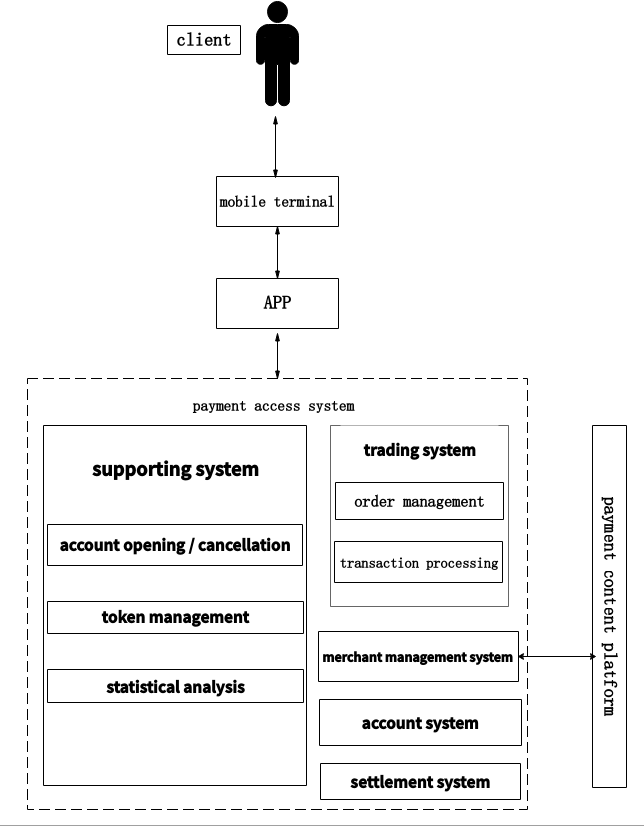
\includegraphics[scale=0.44]{erweimazhifu.png}}
\caption{App payment.}
\label{fig}
\end{figure}
\subsection{Through email}
PayPal is a Web-based e-commerce
business that allows money transfers and
payments to be made through the
Internet. It offers a secure method to
transfer funds between individuals or
business electronically. A special feature
of PayPal is that it does not transmit any
financial information over the Internet as
a bank would do. It is similar to an escrow
service as PayPal acts as the middleman
holder of the money between both parties
involved in a transaction.
In this paper I will focus on the specific
case of Cross-Site Scripting attacks (XSS)
against the security of web applications.
The XSS attack is very similar to SQL
Injection due to the fact that both attacks
inject code into the web application that
poses a threat. A study documented by
Symantec in 2007 showed that roughly
84 of websites are susceptible to cross
site scripting.

PayPal uses the public key cryptography
technology to encrypt your PayPal button
created from your account that is used in
a website.
Public key cryptography provides a way to
prove the identity in the online world. This
cryptographic algorithm uses two keys(public-key and private-key) which are
bits of data that are mathematically
related to one another. This type of
cryptographic algorithm only works only if
you keep the private key confidential,
while the public key can be made
available. The public keys are distributed
inside a digital certificate.
Digital certificates represents a file that
contains information about the public key
(name of the company that owns the
public key, the third party company that
distributed
the
certificate
and
the
certificate expiration date) and the key
itself. The third party involved in signing
the certificate is referred as a certificate
authority (CA). The CA signs the digital
certificate, and the consumers can
validate that the public key is valid by
using the public certificate of the CA to
verify the digital signature.

Even though you can generate an
encrypted PayPal button either from your
PayPal account or through the PayPal API,
many websites still use the standard HTML form for a Buy Now button or
Subscription button.
The code for the encrypted PayPal button
is presented in the image below.
You can see in Figure 1 that the input with
the name $hosted_button_id$ holds the
encrypted value for the product. This
includes the business name. item name,
price, currency shipping and tax values
entered in PayPal.

This type of PayPal button is secure
because it does not display any
information about the merchant or about
the item itself.
Another type of PayPal button is the one
where you can enter all the variables in
plaintext as seen below (Figure 2).

In Figure 2 you can see that the personal
information about your account is now
visible: business (the merchant account),
amount (the price of the item), first
name, last name, address 1, address 2
city, zip (information about the buyer).
All the above information is in plaintext
and can be easily altered for malicious
intents.

For example using a man-in-the-middle
attack as seen in Figure 3, the attacker
intercepts the communication between
the victim and the Web Server. Using
different techniques, the attacker can split
the original connection into two new
connections, one between the victim and
the attacker and the other between the
attacker and the Web Server. Once the
connection is intercepted, the attacker
can read and alter the data from the
intercepted connection. Once the attacker
intercepts the connection he can alter the
merchant account by adding his own

user’s browser allows an attacker to
perform the following types of attack:
Cookie theft: the attacker can access
the victim’s cookies associated with
the website, send them to his own
server and use them to extract
sensitive information like session ID,
which can be used to enter PayPal’s
website (PayPal uses cookies when a
user loges in with his account) as
though he was the actual owner of the
account
 
 Keylogging: the attacker can register
a keyboard event listener, and then
send all of the user’s keystrokes to his
own server, potentially recording
personal or financial information
 Phishing: the attacker can insert a
fake login form into the page, set the
form’s action attribute to target his
own server and then trick the user
into submitting sensitive information.
For security purposes PayPal introduced
an option for using a PayPal Security Key
during the login process. This security
measure is actually an OTP authentication
system
that
generates
a
random
temporary security code (which is
displayed on the PayPal Security Key
card) that must be used together with the
account’s holder username and password
to complete the sign in process.
is ignored and therefore the attack was
successful.
Further,
the
attackers
establish a separate HTTPS connection
with the server to complete the request,
and the result of the response is delivered
to the victim’s browser. This gives the
attackers full control over the SSL traffic
and
helps
them
steal
personal
information. Since the attackers are not
breaking the request-response chain, this
kind of attack becomes tough to detect
the data theft.
2.3.1 NSA Man in the middle
NSA (National Security Agency) is known
for using man in the middle attack.
Because NSA has a secret partnership
with the US telecoms companies, NSA
placed secret servers at key places in the
internet
backbone.
This
placement

ensured that they can react faster then
any other websites can. Exploiting these
speed differences these servers could
impersonate a visited website to the
victim before the legitimate website could
respond, thereby tricking the victim into
thinking they are on the right website.
This kind of attack is very difficult to
execute for any other attackers because it
requires a privileged position in the
internet backbone. NSA uses these fast
servers to execute a packet injection
attack that redirects the victim to one of
the NSA servers.
2.3 The SSL Man in the middle attack
In this case, the attackers intrude into the
network and establish a successful man in
the middle connection. The attackers can
watch the HTTPS traffic and wait for the
targeted website to respond to some
browsers HTTPS request. When a browser
sends a HTTPS request, the server
responds by sending its digital certificate
as part of the SSL handshake protocol. At
this moment, the attackers can grab this
certificate
and
note
down
various
information
as
the
domain
name,
expiration date etc. The attackers can
now create their self-signed certificate
using the information from above. From
this point forward, the attackers intercept
each browser request and respond with
the fake certificate. As a normal response
to this situation, the browser pops up a
warning to the user, which in most cases
2.4 Packet Crafting
Packet crafting is a task that is
methodically carried out to penetrate into
a network’s infrastructure. There are four
steps involved in crafting a packet:
 Packet assembly;
 Packet editing;
 Packet playing;
 Packet analysis.
2.4.1 Paced assembly
This is the first step in the crafting
process, where an attacker decides which
network needs to be cracked, tries to
gather possible vulnerability information
and creates the packets to be sent. The
packet is then checked for accuracy,
especially to ensure that the attack is as
“invisible” on the network as possible, to
go undetected.

user’s browser allows an attacker to
perform the following types of attack:
 Cookie theft: the attacker can access
the victim’s cookies associated with
the website, send them to his own
server and use them to extract
sensitive information like session ID,
which can be used to enter PayPal’s
website (PayPal uses cookies when a
user loges in with his account) as
though he was the actual owner of the
account
 Keylogging: the attacker can register
a keyboard event listener, and then
send all of the user’s keystrokes to his
own server, potentially recording
personal or financial information
 Phishing: the attacker can insert a
fake login form into the page, set the
form’s action attribute to target his
own server and then trick the user
into submitting sensitive information.
For security purposes PayPal introduced
an option for using a PayPal Security Key
during the login process. This security
measure is actually an OTP authentication
system
that
generates
a
random
temporary security code (which is
displayed on the PayPal Security Key
card) that must be used together with the
account’s holder username and password
to complete the sign in process.
is ignored and therefore the attack was
successful.
Further,
the
attackers
establish a separate HTTPS connection
with the server to complete the request,
and the result of the response is delivered
to the victim’s browser. This gives the
attackers full control over the SSL traffic
and
helps
them
steal
personal
information. Since the attackers are not
breaking the request-response chain, this
kind of attack becomes tough to detect
the data theft.
2.3.1 NSA Man in the middle
NSA (National Security Agency) is known
for using man in the middle attack.
Because NSA has a secret partnership
with the US telecoms companies, NSA
placed secret servers at key places in the
internet
backbone.
This
placement
ensured that they can react faster then
any other websites can. Exploiting these
speed differences these servers could
impersonate a visited website to the
victim before the legitimate website could
respond, thereby tricking the victim into
thinking they are on the right website.
This kind of attack is very difficult to
execute for any other attackers because it
requires a privileged position in the
internet backbone. NSA uses these fast
servers to execute a packet injection
attack that redirects the victim to one of
the NSA servers.
2.3 The SSL Man in the middle attack
In this case, the attackers intrude into the
network and establish a successful man in
the middle connection. The attackers can
watch the HTTPS traffic and wait for the
targeted website to respond to some
browsers HTTPS request. When a browser
sends a HTTPS request, the server
responds by sending its digital certificate
as part of the SSL handshake protocol. At
this moment, the attackers can grab this
certificate
and
note
down
various
information
as
the
domain
name,
expiration date etc. The attackers can
now create their self-signed certificate
using the information from above. From
this point forward, the attackers intercept
each browser request and respond with
the fake certificate. As a normal response
to this situation, the browser pops up a
warning to the user, which in most cases
2.4 Packet Crafting
Packet crafting is a task that is
methodically carried out to penetrate into
a network’s infrastructure. There are four
steps involved in crafting a packet:
 Packet assembly;
 Packet editing;
 Packet playing;
 Packet analysis.
2.4.1 Paced assembly
This is the first step in the crafting
process, where an attacker decides which
network needs to be cracked, tries to
gather possible vulnerability information
and creates the packets to be sent. The
packet is then checked for accuracy,
especially to ensure that the attack is as
“invisible” on the network as possible, to
go undetected.
\section{offline payment technologies}
Offline payment is a payment method that is very widely used and very convenient to use. In China today, this type of payment can be seen everywhere, from large shopping malls to small supermarket chains. Even in the underground shopping malls with poor network signals, the surrounding areas of the city, and even tourist attractions in the mountains, as long as a mobile phone, you can pay. The most prominent feature is that the paying party do not need connecting to the Internet, which means only one party need communicate with the payment server.


\subsection{Time-Based One-Time Password:The key to offline payment}
\subsection{IC card and NFC payment}
\subsection{Mobile phone imitate IC card}
With the gradual deployment of Android Pay, Apple Pay and Samsung Pay, mobile payments have returned to the public eye and the comparative articles on several types of payment have not been uncommon in recent days. This article mainly discusses the similarities and differences between several payment methods from a technical point of view.
\\

Apple Pay and Android Pay each serve as a system-level payment application (Apple Pay by iOS, Android Pay by Android), not only play the role of application, but also has a God perspective, as a system feature for other applications developers A unified payment gateway. In other words, other shopping and service applications can invoke APIs of Apple Pay or Android Pay in the development code to charge consumers, for example, purchasing a movie ticket. Before the application is almost always linked to VISA or MasterCard online payment allows users to fill in the cardholder name, card number, expiration date, code and other safety information, each time you have to fill in the shopping (the site should not and can not be saved), or combined with OTP (one-time password) certification, This is a hassle and a safety hazard (previously PC-based cookies were hacked, or consumer websites saved user-card information, such as previous Ctrip, resulting in theft of credit card information); application developers can now call Pay, allowing users to choose their own credit card has been added to pay, users do not need to fill in a form, a key shopping, the real charge to pay to do.\\

Relative to the online payment (in short, that is connected with the Internet, the payment of data through the network transmission), offline payment is a physical payment, you need a terminal device chargeback, in most cases, POS machines. In order to replace the traditional credit card with credit card spending, NFC + Pay way allows consumers to use a cell phone, rather than a variety of cards for "flash" consumption. Pay only needs the POS machine to support NFC without any other modification. Therefore, offline entity merchants accept this payment method exactly as the acceptance of non-connected bank cards such as MasterCard Pay Pass, Visa Pay Wave, China Union Pay Flash Quick Pass , There is no promotion barriers, but also to speed up the deployment of wireless POS machines coupled with a heavy weight.

\subsubsection{sumsung pay}
\subsubsection{Android pay}
\subsubsection{apple pay}

\section{Disscusion and security comparison}
\section{Conclusion}
The conclusion goes here.





% if have a single appendix:
%\appendix[Proof of the Zonklar Equations]
% or
%\appendix  % for no appendix heading
% do not use \section anymore after \appendix, only \section*
% is possibly needed

% use appendices with more than one appendix
% then use \section to start each appendix
% you must declare a \section before using any
% \subsection or using \label (\appendices by itself
% starts a section numbered zero.)
%


\appendices
\section{Proof of the First Zonklar Equation}
Appendix one text goes here.

% you can choose not to have a title for an appendix
% if you want by leaving the argument blank
\section{}
Appendix two text goes here.


% use section* for acknowledgment
\section*{Acknowledgment}


The authors would like to thank...


% Can use something like this to put references on a page
% by themselves when using endfloat and the captionsoff option.
\ifCLASSOPTIONcaptionsoff
  \newpage
\fi



% trigger a \newpage just before the given reference
% number - used to balance the columns on the last page
% adjust value as needed - may need to be readjusted if
% the document is modified later
%\IEEEtriggeratref{8}
% The "triggered" command can be changed if desired:
%\IEEEtriggercmd{\enlargethispage{-5in}}

% references section

% can use a bibliography generated by BibTeX as a .bbl file
% BibTeX documentation can be easily obtained at:
% http://mirror.ctan.org/biblio/bibtex/contrib/doc/
% The IEEEtran BibTeX style support page is at:
% http://www.michaelshell.org/tex/ieeetran/bibtex/
%\bibliographystyle{IEEEtran}
% argument is your BibTeX string definitions and bibliography database(s)
%\bibliography{IEEEabrv,../bib/paper}
%
% <OR> manually copy in the resultant .bbl file
% set second argument of \begin to the number of references
% (used to reserve space for the reference number labels box)
\begin{thebibliography}{1}

\bibitem{IEEEhowto:kopka}
H.~Kopka and P.~W. Daly, \emph{A Guide to \LaTeX}, 3rd~ed.\hskip 1em plus
  0.5em minus 0.4em\relax Harlow, England: Addison-Wesley, 1999.
 
\bibitem{IEEEhowto:kopka}
Agbinya J I, Masihpour M. \emph{Power Equations and Capacity Performance of Magnetic Induction Communication Systems[J]}. Wireless Personal Communications, 2012, 64(4):831-845.
\bibitem{IEEEhowto:kopka}
Timalsina S K, Moh S. A review on NFC and NFC-based mobile payment solution[J]. Journal of Next Generation Information Technology, 2012, 3(4):35-44.
\bibitem{IEEEhowto:kopka}
NFC Forum, “\emph{White paper on ’smart posters’},” Tech. Rep., Apr. 2011.
\bibitem{IEEEhowto:kopka}
NFC Forum, \emph{“White paper on ’essentials for successful NFC mobile ecosystem’,}” Tech. Rep., Oct.
2008.
\bibitem{IEEEhowto:kopka}
NFC Forum, \emph{“White paper on ’the keys to truly interoperable communications’},” Tech. Rep., Oct.2007.
\bibitem{IEEEhowto:kopka}
R. Steffen, J. Prei andinger, T. Scho andllermann, A. Mu andller, and I. Schnabel, \emph{“Near field communication (NFC) in an automotive environment,}” Proc. of 2010 Second International Workshop on Near Field Communication (NFC), pp. 15-20, Apr. 2010.
\bibitem{IEEEhowto:kopka}
E. Haselsteiner and K. Breitfu, \emph{“Security in near field communication (NFC),}” Proc. of Workshop on RFID security, 2006.
\bibitem{IEEEhowto:kopka}
E. Haselsteiner and K. Breitfu, \emph{“Security in near field communication (NFC),}” Proc. of Workshop
on RFID security, 2006.
\end{thebibliography}

% biography section
% 
% If you have an EPS/PDF photo (graphicx package needed) extra braces are
% needed around the contents of the optional argument to biography to prevent
% the LaTeX parser from getting confused when it sees the complicated
% \includegraphics command within an optional argument. (You could create
% your own custom macro containing the \includegraphics command to make things
% simpler here.)
%\begin{IEEEbiography}[{\includegraphics[width=1in,height=1.25in,clip,keepaspectratio]{mshell}}]{Michael Shell}
% or if you just want to reserve a space for a photo:

\begin{IEEEbiography}{Michael Shell}
Biography text here.
\end{IEEEbiography}

% if you will not have a photo at all:
\begin{IEEEbiographynophoto}{John Doe}
Biography text here.
\end{IEEEbiographynophoto}

% insert where needed to balance the two columns on the last page with
% biographies
%\newpage

\begin{IEEEbiographynophoto}{Jane Doe}
Biography text here.
\end{IEEEbiographynophoto}

% You can push biographies down or up by placing
% a \vfill before or after them. The appropriate
% use of \vfill depends on what kind of text is
% on the last page and whether or not the columns
% are being equalized.

%\vfill

% Can be used to pull up biographies so that the bottom of the last one
% is flush with the other column.
%\enlargethispage{-5in}



% that's all folks
\end{document}


